\documentclass[11pt]{beamer}
% PACKAGES =====================================================================
\usepackage[utf8]{inputenc}
\usepackage{hyperref}
\usepackage{amsmath}
\usepackage{amsfonts}
\usepackage{amssymb}
\usepackage{graphicx}
\usepackage{algorithmic}
\usepackage{algorithm}
\usepackage{wrapfig}
\usepackage{subcaption}
\usepackage{tcolorbox}

% THEMES AND BEAMER SETTINGS ===================================================
% \usetheme{Madrid}
\graphicspath{{.}}


% These are Heniz's notations. 
\newcommand{\To}{\ensuremath{\rightrightarrows}}
\newcommand{\GX}{\ensuremath{\Gamma}}
\newcommand{\mal}{\ensuremath{\mathfrak{m}}}
\newcommand{\mumu}{\ensuremath{{\mu\mu}}}
\newcommand{\paver}{\ensuremath{\mathcal{P}}}
\newcommand{\ZZZ}{\ensuremath{{X \times X^*}}}
\newcommand{\RRR}{\ensuremath{{\RR \times \RR}}}
\newcommand{\todo}{\hookrightarrow\textsf{TO DO:}}

\newcommand{\emp}{\ensuremath{\varnothing}}
%\newcommand{\la}{\ensuremath{\langle}}
%\newcommand{\ra}{\ensuremath{\rangle}}
\newcommand{\infconv}{\ensuremath{\mbox{\small$\,\square\,$}}}
\newcommand{\pscal}{\ensuremath{\scal{\cdot}{\cdot}}}
\newcommand{\Tt}{\ensuremath{\mathfrak{T}}}
\newcommand{\YY}{\ensuremath{\mathcal Y}}
\newcommand{\XX}{\ensuremath{\mathcal X}}
\newcommand{\HH}{\ensuremath{\mathcal H}}
\newcommand{\XP}{\ensuremath{\mathcal X}^*}
\newcommand{\st}{\ensuremath{\;|\;}}
\newcommand{\zeroun}{\ensuremath{\left]0,1\right[}}

\newcommand{\lev}[1]{\ensuremath{\mathrm{lev}_{\leq #1}\:}}
\newcommand{\moyo}[2]{\ensuremath{\sideset{_{#2}}{}{\operatorname{}}\!#1}}
\newcommand{\pair}[2]{\left\langle{{#1},{#2}}\right\rangle}
%\newcommand{\scal}[2]{\left.\left\langle{#1}\:\right| {#2}  \right\rangle}
\newcommand{\scal}[2]{\langle{{#1},{#2}}\rangle}
\newcommand{\Scal}[2]{\left\langle{{#1},{#2}}\right\rangle}
%\newcommand{\scal}[2]{\braket{ {#1},{#2}}}

\newcommand{\yosida}{\ensuremath{ \; {}^}}
\newcommand{\exi}{\ensuremath{\exists\,}}
\newcommand{\GG}{\ensuremath{\mathcal G}}
\newcommand{\RR}{\ensuremath{\mathbb R}}
\newcommand{\SSS}{\ensuremath{\mathbb S}}
\newcommand{\CC}{\ensuremath{\mathbb C}}
\newcommand{\Real}{\ensuremath{\mathrm{Re}\,}}
\newcommand{\ii}{\ensuremath{\mathrm i}}
\newcommand{\RP}{\ensuremath{\left[0,+\infty\right[}}
\newcommand{\RPX}{\ensuremath{\left[0,+\infty\right]}}
\newcommand{\RPP}{\ensuremath{\,\left]0,+\infty\right[}}
\newcommand{\RX}{\ensuremath{\,\left]-\infty,+\infty\right]}}
\newcommand{\RXX}{\ensuremath{\,\left[-\infty,+\infty\right]}}
\newcommand{\KK}{\ensuremath{\mathbb K}}
\newcommand{\NN}{\ensuremath{\mathbb N}}
\newcommand{\nnn}{\ensuremath{{n \in \NN}}}
\newcommand{\thalb}{\ensuremath{\tfrac{1}{2}}}
\newcommand{\zo}{\ensuremath{{\left]0,1\right]}}}
\newcommand{\lzo}{\ensuremath{{\lambda \in \left]0,1\right]}}}
%\newcommand{\toppsepp}{\setlength{\partopsep}{-5pt}}
\newcommand{\menge}[2]{\big\{{#1} \mid {#2}\big\}}
\newcommand{\pfrac}[2]{\ensuremath{\mathlarger{\tfrac{#1}{#2}}}}


% MATH OPERATORS ===============================================================
% \newcommand{\monos}{\ensuremath{\mathcal M}}
\newcommand{\DD}{\operatorname{dom}f}
\newcommand{\IDD}{\ensuremath{\operatorname{int}\operatorname{dom}f}}
\newcommand{\CDD}{\ensuremath{\overline{\operatorname{dom}}\,f}}
\newcommand{\clspan}{\ensuremath{\overline{\operatorname{span}}}}
\newcommand{\cone}{\ensuremath{\operatorname{cone}}}
\newcommand{\dom}{\ensuremath{\operatorname{dom}}}
\newcommand{\closu}{\ensuremath{\operatorname{cl}}}
\newcommand{\cont}{\ensuremath{\operatorname{cont}}}
\newcommand{\mons}{\ensuremath{\mathcal{A}}}
\newcommand{\gra}{\ensuremath{\operatorname{gra}}}
\newcommand{\epi}{\ensuremath{\operatorname{epi}}}
\newcommand{\prox}{\ensuremath{\operatorname{Prox}_{\mu}}}
\newcommand{\hprox}{\ensuremath{\operatorname{prox}}}
\newcommand{\intdom}{\ensuremath{\operatorname{int}\operatorname{dom}}\,}
\newcommand{\inte}{\ensuremath{\operatorname{int}}}
\newcommand{\sri}{\ensuremath{\operatorname{sri}}}
\newcommand{\reli}{\ensuremath{\operatorname{ri}}}
\newcommand{\cart}{\ensuremath{\mbox{\LARGE{$\times$}}}}


\newcommand{\average}{\ensuremath{\mathcal{R}_{\mu}({\bf A},{\boldsymbol \lambda})}}
\newcommand{\averagebar}{\ensuremath{\mathcal{R}_{1}({\bf A},\bar{\lambda})}}
\newcommand{\averageonelambda}{\ensuremath{\mathcal{R}({\bf A},{\boldsymbol \lambda})}}
\newcommand{\averageonehalf}{\ensuremath{\mathcal{R}_{1}(A,1/2)}}
\newcommand{\averageinverse}{\ensuremath{\mathcal{R}_{\mu^{-1}}({\bf A}^{-1},{\boldsymbol \lambda})}}
\newcommand{\averageoneinverse}{\ensuremath{\mathcal{R}({\bf A}^{-1},{\boldsymbol \lambda})}}
\newcommand{\averagef}{\ensuremath{\mathcal{P}_{\mu}(f,\lambda)}}
\newcommand{\averagefone}{\ensuremath{\mathcal{P}_{1}(f,\lambda)}}
\newcommand{\averagefd}{\ensuremath{\mathcal{P}_{\mu}((f_{1},\ldots, f_{n}),(\lambda_{1},\ldots, \lambda_{n}))}}
\newcommand{\averagefik}{\ensuremath{\mathcal{P}_{\mu_{k}}((f_{1,k},\ldots,f_{n,k}),
(\lambda_{1,k},\ldots,\lambda_{n,k}))}}
\newcommand{\averagesub}{\ensuremath{\mathcal{R}_{\mu}(\partial f,\lambda)}}
\newcommand{\res}{\ensuremath{\mathcal{R}_{\mu}}}
\newcommand{\resmuk}{\ensuremath{\mathcal{R}_{\mu_{k}}}}
\newcommand{\newres}{\ensuremath{\mathcal{R}}}
\newcommand{\resmualpha}{\ensuremath{\mathcal{R}_{\alpha\mu}}}
\newcommand{\averageone}{\ensuremath{\mathcal{R}_{1}}}
\newcommand{\harm}{\ensuremath{\mathcal{H}(A,\lambda)}}
\newcommand{\arithmetic}{\ensuremath{\mathcal{A}(A,\lambda)}}

\newcommand{\WC}{\ensuremath{{\mathfrak W}}}
\newcommand{\SC}{\ensuremath{{\mathfrak S}}}
\newcommand{\card}{\ensuremath{\operatorname{card}}}
\newcommand{\bd}{\ensuremath{\operatorname{bdry}}}
\newcommand{\ran}{\ensuremath{\operatorname{ran}}}
\newcommand{\rec}{\ensuremath{\operatorname{rec}}}
\newcommand{\rank}{\ensuremath{\operatorname{rank}}}
\newcommand{\kernel}{\ensuremath{\operatorname{ker}}}
\newcommand{\conv}{\ensuremath{\operatorname{conv}}}
\newcommand{\segh}{\ensuremath{\operatorname{seg}}}
\newcommand{\boxx}{\ensuremath{\operatorname{box}}}
\newcommand{\clconv}{\ensuremath{\overline{\operatorname{conv}}\,}}
\newcommand{\cldom}{\ensuremath{\overline{\operatorname{dom}}\,}}
\newcommand{\clran}{\ensuremath{\overline{\operatorname{ran}}\,}}
\newcommand{\Nf}{\ensuremath{\nabla f}}
\newcommand{\NNf}{\ensuremath{\nabla^2f}}
\newcommand{\Fix}{\ensuremath{\operatorname{Fix}}}
\newcommand{\FFix}{\ensuremath{\overline{\operatorname{Fix}}\,}}
\newcommand{\aFix}{\ensuremath{\widetilde{\operatorname{Fix}\,}}}
\newcommand{\Id}{\ensuremath{\operatorname{Id}}}
\newcommand{\Max}{\ensuremath{\operatorname{max}}}
\newcommand{\Bb}{\ensuremath{\mathfrak{B}}}
\newcommand{\BB}{\ensuremath{\mathbb{B}}}
\newcommand{\Fb}{\ensuremath{\overrightarrow{\mathfrak{B}}}}
\newcommand{\Fprox}{\ensuremath{\overrightarrow{\operatorname{prox}}}}
\newcommand{\Bprox}{\ensuremath{\overleftarrow{\operatorname{prox}}}}
\newcommand{\Bproj}{\ensuremath{\overleftarrow{\operatorname{P}}}}
\newcommand{\Ri}{\ensuremath{\mathfrak{R}_i}}
\newcommand{\Dn}{\ensuremath{\,\overset{D}{\rightarrow}\,}}
\newcommand{\nDn}{\ensuremath{\,\overset{D}{\not\rightarrow}\,}}
\newcommand{\weakly}{\ensuremath{\,\rightharpoonup}\,}
\newcommand{\weaklys}{\ensuremath{\,\overset{*}{\rightharpoonup}}\,}
\newcommand{\gr}{\ensuremath{\operatorname{gra}}}
\newcommand{\g}{\ensuremath{\,\overset{g}{\rightarrow}}\,}
\newcommand{\p}{\ensuremath{\,\overset{p}{\rightarrow}}\,}
\newcommand{\e}{\ensuremath{\,\overset{e}{\rightarrow}}\,}
\newcommand{\Tbar}{\ensuremath{\overline{T}}}
\newcommand{\n}{\ensuremath{\,\overset{n}{\rightarrow}}\,}

\newcommand{\minf}{\ensuremath{-\infty}}
\newcommand{\pinf}{\ensuremath{+\infty}}
\renewcommand{\iff}{\ensuremath{\Leftrightarrow}}
% \renewcommand{\phi}{\ensuremath{\varphi}}
%\newcommand{\Real}{\ensuremath{\mathrm{Re}\,}}
\newcommand{\negent}{\ensuremath{\operatorname{negent}}}
\newcommand{\neglog}{\ensuremath{\operatorname{neglog}}}
\newcommand{\halb}{\ensuremath{\tfrac{1}{2}}}
\newcommand{\bT}{\ensuremath{\mathbf{T}}}
\newcommand{\bX}{\ensuremath{\mathbf{X}}}
\newcommand{\bL}{\ensuremath{\mathbf{L}}}
\newcommand{\bD}{\ensuremath{\boldsymbol{\Delta}}}
\newcommand{\bc}{\ensuremath{\mathbf{c}}}
\newcommand{\by}{\ensuremath{\mathbf{y}}}
\newcommand{\bx}{\ensuremath{\mathbf{x}}}
\newcommand{\bA}{{\bf A}}
\newcommand{\Other}{Indeterminate }
\newcommand{\other}{indeterminate }


%%% Raf's stuff  ===============================================================
\newcommand{\al}{\alpha}
\newcommand{\la}{\lambda}
\newcommand{\La}{\Lambda}
\newcommand{\pluss}{{\hskip1pt \raise1pt\vbox{\hrule width6pt \vskip1pt
\hrule width6pt}\kern-4pt{\lower1pt\hbox{\vrule height6pt \kern1pt\vrule
height6pt}}\hskip5pt}}
\newcommand{\timess}{\star}
\newcommand{\argmax}{\mathop{\rm argmax}\limits}
\newcommand{\argmin}{\mathop{\rm argmin}\limits}
\newcommand{\product}{\langle\cdot,\cdot\rangle}
\newcommand{\im}{\mathrm{Im}}
\newcommand{\multival}{\ensuremath{X\to 2^{X^*}}}
\newcommand{\SX}{\ensuremath{2^{X^*}}} % IMPORT WANG'S LATEX CUSTOM COMMANDS. 
\setbeamertemplate{theorems}[numbered] % ADD NUMBERING TO ALL AMS THEOREMS. 
\setbeamertemplate{footline}[frame number] % ADD PAGE NUMBERS ON BOTTOM. 
% BIB STYLES SETTINGS ----------------------------------------------------------
\setbeamerfont{bibliography item}{size=\footnotesize}
\setbeamerfont{bibliography entry author}{size=\footnotesize}
\setbeamerfont{bibliography entry title}{size=\footnotesize}
\setbeamerfont{bibliography entry location}{size=\footnotesize}
\setbeamerfont{bibliography entry note}{size=\footnotesize}
% \setbeamercovered{transparent}  % GREY OUT PAUSED FUTURE ITEMS IN SLID. 
\setbeamertemplate{navigation symbols}{} 


% SLIDE INFORMATION ============================================================
\author{Hongda Li}
\title[Thesis Proposal Talk]{First Order Nonsmooth Optimization: Catalyst Acceleration and Unifying Nesterov's Acceleration}
% \newcommand{\email}{lalala@lala.la}
\institute[UBCO]{
    University of British Columbia Okanagan
}
\date{\today}
\subject{Nesterov's acceleration and its applications}


% SLIDES ELEMENTS CUSTOMIZATIONS ===============================================
\theoremstyle{definition}
\newtheorem{remark}{Remark}[section]
\newtheorem{assumption}{Assumption}[section]
\newtheorem{proposition}{Proposition}[section]
\bibliographystyle{siam}


% DOCUMENTS STARTS =============================================================
\begin{document}
\begin{frame}
    \titlepage
\end{frame}
\begin{frame}{Overview}
    This talk will be based on the content of our draft paper and selected content of the Catalyst Meta Acceleration Framework. 
    Our preprint: 
    \begin{enumerate}
        \item X. Wang and H. Li, \textit{A Parameter Free Accelerated Proximal Gradient Method Without Restarting}, preprint, (2025).
    \end{enumerate}
    Catalyst Meta Acceleration:  
    \begin{enumerate}
        \item H. Lin, J. Mairal and Z. Harchaoui, \textit{A universal catalyst for first-order optimization}, in NISP, vol. 28, (2015). 
        \item \underline{\hspace{4em}}, \textit{Catalyst acceleration for first-order convex optimization: from theory to practice}, JMLR, 18 (2018), pp. 1–54.
    \end{enumerate}
\end{frame}

\begin{frame}[allowframebreaks]{ToC}
    \tableofcontents
\end{frame}


\section{Introduction}
    \subsection{Notations and preliminaries}
        \begin{frame}{Notations and preliminaries}
            Throughout this talk, let $\RR^n$ be the ambient space equipped with Euclidean inner product and norm. 
            We consider 
            \begin{align}\label{eqn:additive-comp-obj}
                \min_{x \in \RR^n} \left\lbrace
                    F(x):= f(x) + g(x)
                \right\rbrace.
            \end{align}
            Unless specified, assume: 
            \begin{enumerate}
                \item $f:\RR^n \rightarrow \RR$ is $L$-Lipscthiz smooth $\mu \ge 0$ strongly convex, 
                \item $g:\RR^n \rightarrow \overline \RR$ is closed convex proper. 
                \item Minimum exists $F^* = \min_{x\in \RR^n}\{f(x) + g(x)\}$ and minimizer exists. 
            \end{enumerate}
        \end{frame}
        \begin{frame}{Notations and preliminaries}
            \begin{definition}[Proximal gradient operator]\label{def:proximal-gradient-operator}
                Define the proximal gradient operator $T_L$ on all $y \in \RR^n$: 
                \begin{align*}
                    T_L y := \argmin_{x \in \RR^n} \left\lbrace
                        g(x) + f(y) + \langle \nabla f(y), x - y\rangle 
                        + \frac{L}{2}\Vert x- y \Vert^2
                    \right\rbrace. 
                \end{align*}
            \end{definition}
            \begin{definition}[Gradient mapping operator]\label{def:gradient-mapping-operator}
                % Take $F := f + g$ as defined in this section. 
                Define the gradient mapping operator $\mathcal G_L$ on all $y \in \RR^n$: 
                \begin{align*}
                    \mathcal G_L (y):= L(y - T_L y). 
                \end{align*}
            \end{definition}
        \end{frame}
        \begin{frame}{Proximal gradient inequality}
            \begin{lemma}[The proximal gradient inequality]\label{thm:prox-grad-ineq}
                % Take $F:= f + g$ as defined in this section. 
                For all $y \in \RR^n$, $x \in \RR^n$, it has: 
                {\scriptsize
                \begin{align*}
                    F(x)  - F(T_Ly) - \langle L(y - T_Ly), x - y\rangle
                    - \frac{\mu}{2}\Vert x - y\Vert^2 - \frac{L}{2}\Vert y - T_Ly\Vert^2 
                    &\ge 0. 
                \end{align*}
                }
            \end{lemma}
            This lemma is crucial to developing results in our current draft paper. 
        \end{frame}
        \begin{frame}{Nesterov's estimating sequence example}
            \begin{definition}[Nesterov's estimating sequence]\label{def:nes-est-seq}
                For all $k \ge 0$, let $\phi_k : \RR^n \rightarrow\RR$ be a sequence of functions. 
                We call this sequence of functions a Nesterov's estimating sequence when it satisfies conditions: 
                \begin{enumerate}
                    \item There exists another sequence $(x_k)_{k \ge 0}$ such that for all $k \ge 0$ it has $F(x_k) \le \phi_k^*: =\min_{x}\phi_k(x)$. 
                    \item There exists a sequence of $(\alpha_k)_{k \ge 0}$ where $\alpha_k \in (0, 1)\; \forall k \ge0 $ such that for all $x \in \RR^n$ it has $\phi_{k + 1}(x) - \phi_k(x) \le - \alpha_k(\phi_k(x) - F(x))$. 
                \end{enumerate}
            \end{definition}
            The technique is widespread in the literatures and it's used to derive the convergence rate of acceleration on first order method, and the numerical algorithm itself. It is a two birds one stone technique. 
        \end{frame}
        \begin{frame}{Our works on R-WAPG}
            Recall the Nesterov's acceleration has momentum extrapolation updates on $y_{k + 1} = x_{k + 1} + \theta_{k + 1}(x_{k + 1} - x_k)$. 
            We proposed the idea of R-WAPG, a generic method that: 
            \begin{enumerate}
                \item Describe for momentum sequences that doesn't follow Nesterov's rules.
                \item Unifies the convergence rate analysis for several Euclidean variants of the FISTA method. 
                \item A parameter free numerical algorithm: ``Free R-WAPG'' method that has competitive numerical performance in practical settings without restarting. 
            \end{enumerate}
            Our work is inspired by considering Nesterov's estimating sequence where $F(x_k) + R_k = \phi_k^*$. 
        \end{frame}
        \begin{frame}{Introducing Catalyst Part I}
            \begin{block}{Introducing Catalyst}
                Let $F:\RR \rightarrow \overline \RR$ be $\mu \ge 0$ strongly convex and closed. 
                Let the initial estimate be $x_0 \in \RR^n$, fix parameters $\kappa > 0$ and $\alpha_0 \in (0, 1]$. 
                {\small 
                \begin{tcolorbox}
                    Initialize $x_0 = y_0$. Then the algorithm generates $(x_k, y_k)_{k\ge 0}$ for all $k \ge 1$ such that: 
                    \begin{align*}
                        & \text{find } x_k \approx \argmin_{x \in \RR^n} \left\lbrace F(x) + (\kappa/2)\Vert x - y_{k - 1}\Vert^2\right\rbrace, 
                        \\
                        & \text{find } \alpha_k \in (0, 1) \text{ such that } \alpha_k^2 = (1 - \alpha_k)\alpha_{k - 1}^2 + (\mu/(\mu + \kappa))\alpha_k,
                        \\
                        & 
                        y_{k} = x_k + \frac{\alpha_{k - 1}(1 - \alpha_{k - 1})}{\alpha_{k - 1}^2 + \alpha_k}(x_k - x_{k - 1}). 
                    \end{align*}
                \end{tcolorbox}
                }
            \end{block}
            We will return to this in the later slides. 
        \end{frame}
        \begin{frame}{Introducing Catalyst Part II}
            Catalyst by Lin, et al. \cite{lin_catalyst_2018, lin_universal_2015} has the theoretical and practical importance: 
            \begin{enumerate}
                \item It's an early attempt at putting accelerated inexact proximal point method into a practical setting. 
                \item It finds application in machine learning and it accelerates the convergence of Variance Reduced Method (A type of incremental method that is not slower than the exact counter part). 
                \item It demonstrates crucial ideas on how prove convergence rate where the evaluation of proximal point method is inexact in the convex settings. 
            \end{enumerate}
        \end{frame}

\section{Content of the draft paper}
    \subsection{The method of R-WAPG and its convergence}
        \begin{frame}{R-WAPG sequences}
            \begin{definition}[R-WAPG sequences]\label{def:rwapg-seq}
                Assume $0 \le \mu < L$. 
                The sequences $(\alpha_k)_{k \ge 0}, (\rho_k)_{k \ge 0}$ are valid for R-WAPG if all the following holds: 
                \begin{align*}
                    \alpha_0 &\in (0, 1], 
                    \\
                    \alpha_k &\in (\mu/L, 1) \quad (\forall k \ge 1), 
                    \\
                    \rho_k &:= \frac{\alpha_{k + 1}^2 - (\mu/L)\alpha_{k + 1}}{(1 - \alpha_{k + 1})\alpha_k^2} \quad \forall (k \ge 0). 
                \end{align*}
                We call $(\alpha_k)_{k \ge 0}, (\rho_k)_{k \ge 0}$ the \textbf{R-WAPG Sequences}. 
            \end{definition}
        \end{frame}
        \begin{frame}{The method of R-WAPG}
            \begin{definition}[Relaxed weak accelerated proximal gradient (R-WAPG)]\label{def:wapg}
                Choose any $x_1 \in \RR^n, v_1 \in \RR^n$. 
                Let $(\alpha_k)_{k \ge0}, (\rho_k)_{k \ge 0}$ be given by Definition \ref{def:rwapg-seq}. 
                The algorithm generates a sequence of vector $(y_k, x_{k + 1}, v_{k + 1})_{k \ge 1}$ for $k\ge 1$ by the procedures:  
                \begin{tcolorbox}
                    For $k=1, 2, 3, \ldots$
                    \begin{align*}
                        \gamma_k &:= \rho_{k -1}L\alpha_{k - 1}^2, 
                        \\
                        \hat \gamma_{k + 1} & := (1 - \alpha_k)\gamma_k + \mu \alpha_k = L\alpha_k^2, 
                        \\
                        y_k &= 
                        (\gamma_k + \alpha_k \mu)^{-1}(\alpha_k \gamma_k v_k + \hat\gamma_{k + 1} x_k), 
                        \\
                        g_k &= \mathcal G_L y_k, 
                        \\
                        v_{k + 1} &= 
                        \hat\gamma^{-1}_{k + 1}
                        (\gamma_k(1 - \alpha_k) v_k - \alpha_k g_k + \mu \alpha_k y_k), 
                        \\
                        x_{k + 1} &= T_L y_k. 
                    \end{align*}    
                \end{tcolorbox}
            \end{definition}
        \end{frame}
        \begin{frame}{Convergence of R-WAPG}
            The convergence claim of the method follows. 
            \begin{proposition}[R-WAPG convergence claim]\label{prop:wagp-convergence}
                Fix any arbitrary $x^* \in \RR^n, N \in \mathbb N$. 
                Let vector sequence $(y_k, v_{k}, x_{k})_{k \ge 1}$ and R-WAPG sequences $\alpha_k, \rho_k$ be given by Definition \ref{def:wapg}. 
                Define $R_1 = 0$ and suppose that for $k = 1, 2, \ldots, N$, we have $R_k$ recursively given by: 
                {\scriptsize
                \begin{align*}
                    R_{k + 1}
                    := 
                    \frac{1}{2}\left(
                        L^{-1} - \frac{\alpha_k^2}{\hat \gamma_{k + 1}}
                    \right)\Vert g_k\Vert^2
                    + 
                    (1 - \alpha_k)
                    \left(
                        \epsilon_k + R_k + 
                        \frac{\mu\alpha_k\gamma_k}{2\hat \gamma_{k + 1}}
                        \Vert v_k - y_k\Vert^2
                    \right). 
                \end{align*}
                }
                Then for all $k = 1, 2, \ldots, N$: 
                {\scriptsize
                \begin{align*}
                    & F(x_{k + 1}) - F(x^*) + \frac{L \alpha_k^2}{2}\Vert v_{k + 1} - x^*\Vert^2
                    \\
                    &\le 
                    \left(
                        \prod_{i = 0}^{k - 1} \max(1, \rho_{i})
                    \right)
                    \left(
                        \prod_{i = 1}^{k} \left(1  - \alpha_i\right)
                    \right)
                    \left(
                        F(x_1) - F(x^*) + \frac{L\alpha_0^2}{2}\Vert v_1 - x^*\Vert^2
                    \right). 
                \end{align*}
                }
            \end{proposition}
        \end{frame}
    \subsection{Equivalent forms of R-WAPG}
        \begin{frame}{Equivalent forms of R-WAPG}
            \begin{enumerate}
                \item Equivalent forms of R-WAPG exists and resembles variants of FISTA in the literatures
                \item We proved the equivalences in our draft papers and the convergence claim from previous applies to all the equivalent forms of R-WAPG which will follow. 
            \end{enumerate}    
        \end{frame}
        \begin{frame}{R-WAPG intermediate form}
            \begin{definition}[R-WAPG intermediate form]\label{def:r-wapg-intermediate}
                Assume $\mu < L$ and let $(\alpha_k)_{k \ge 0}, (\rho_k)_{k \ge 0}$ given by Definition \ref{def:rwapg-seq}. 
                Initialize any $x_1, v_1$ in $\RR^n$. 
                For $k \ge 1$, the algorithm generates sequence of vector iterates $(y_{k}, v_{k + 1}, x_{k + 1})_{k \ge 1}$ by the procedures: 
                {\small
                \begin{tcolorbox}
                    For $k = 1, 2, \ldots$
                    \begin{align*} 
                        & y_{k} = 
                        \left(
                            1 + \frac{L - L\alpha_{k}}{L\alpha_{k} - \mu}
                        \right)^{-1}
                        \left(
                            v_{k + 1} + 
                            \left(\frac{L - L\alpha_{k}}{L\alpha_{k} - \mu} \right) x_{k}
                        \right), 
                        \\
                        & x_{k + 1} = 
                        y_k - L^{-1} \mathcal G_L y_k, 
                        \\
                        & v_{k + 1} = 
                        \left(
                            1 + \frac{\mu}{L \alpha_k - \mu}
                        \right)^{-1}
                        \left(
                            v_k + 
                            \left(\frac{\mu}{L \alpha_k - \mu}\right) y_k
                        \right) - \frac{1}{L\alpha_{k}}\mathcal G_L y_k. 
                    \end{align*}
                \end{tcolorbox}
                }
            \end{definition}
            \pause
            \begin{enumerate}
                \item If, $\mu = 0$, this is Chapter 12 of in Ryu and Yin's Book \cite{ryu_large-scale_2022}, right after Theorem 17.
            \end{enumerate}
        \end{frame}
        \begin{frame}{R-WAPG similar triangle form}
            \begin{definition}[R-WAPG similar triangle form]\label{def:r-wapg-st-form}
            {\small
                Given any $(x_1, v_1)$ in $\RR^n$. 
                Assume $\mu < L$.
                Let the sequence $(\alpha_k)_{k \ge 0}, (\rho_k)_{k\ge 0}$ be given by Definition \ref{def:rwapg-seq}. 
                For $k \ge 1$, the algorithm generates sequences of vector iterates $(y_k, v_{k + 1}, x_{k + 1})_{k \ge 1}$ by the procedures: 
                \begin{tcolorbox}
                    For $k=1, 2, \ldots $
                    {\scriptsize
                    \begin{align*}
                        & y_k = 
                        \left(
                            1 + \frac{L - L\alpha_k}{L\alpha_k - \mu}
                        \right)^{-1}
                        \left(
                            v_k + 
                            \left(\frac{L - L\alpha_k}{L\alpha_k - \mu} \right) x_k
                        \right), 
                        \\
                        & x_{k + 1} = 
                        y_k - L^{-1} \mathcal G_L y_k, 
                        \\
                        & v_{k + 1} = 
                        x_{k + 1} + (\alpha_k^{-1} -1)(x_{k + 1} - x_k). 
                    \end{align*}   
                    } 
                \end{tcolorbox}
            }
            \end{definition}
            \pause
            {\small
            \begin{enumerate}
                \item Equation (2), (3), (4) in \cite{chambolle_convergence_2015} is a similar triangle formulation of FISTA with $\mu = 0$. 
                \item see (3.1, 4.1) in Lee et al. \cite{lee_geometric_2021} and Ahn and Sra \cite{ahn_understanding_2022} for graphical visualization of similar triangle form. 
            \end{enumerate}
            }
        \end{frame}

        \begin{frame}{R-WAPG momentum form}
            \begin{definition}[R-WAPG momentum form]\label{def:r-wapg-momentum-form}
                Given any $y_1 = x_1 \in \RR^n$, and sequences $(\rho_k)_{k \ge 0}, (\alpha_k)_{k\ge 0}$ Definition \ref{def:rwapg-seq}. 
                The algorithm generates iterates $x_{k + 1}, y_{k + 1}$ For $k = 1, 2, \cdots $ by the procedures: 
                {\small
                \begin{tcolorbox}
                    For $k=1, 2,\ldots $
                    \begin{align*}
                        & x_{k + 1} = y_k - L^{-1}\mathcal G_Ly_k, 
                        \\
                        & 
                        y_{k + 1} = 
                        x_{k + 1} + 
                        \frac{\rho_k\alpha_k(1 - \alpha_k)}{\rho_k\alpha_k^2 + \alpha_{k + 1}}(x_{k + 1} - x_k). 
                    \end{align*}    
                \end{tcolorbox}
                }
                In the special case where $\mu = 0$, the momentum term can be represented without parameter $\rho_k$: 
                $$
                    (\forall k \ge 1)\quad \frac{\rho_k\alpha_k(1 - \alpha_k)}{\rho_k\alpha_k^2 + \alpha_{k + 1}} 
                    = \alpha_{k + 1}(\alpha_k^{-1} - 1). 
                $$
            \end{definition}
        \end{frame}

    \subsection{Unified Convergence claim with relaxed Nesterov's sequence}
        \begin{frame}{Summary of our results}
            With the equivalent representations and the convergence claim for relaxed sequence $(\alpha_k)_{k \ge 0}$ of the R-WAPG, we are able to unifies: 
            \begin{enumerate}
                \item Several Euclidean variants of the FISTA algorithm. 
                \item Nontraditional choices of momentum sequences. 
            \end{enumerate}
            The table below summarizes our major results. \begin{table}[H]
            {\tiny
            \begin{tabular}{|l|l|l|l|}
            \hline
                Algorithm & $\mu$ & $\alpha_k, \rho_k$ & $F(x_k) - F^* \le \mathcal O(\cdot)$ 
            \\ \hline
                Definition \ref{def:wapg} & 
                $\mu \ge 0$ &
                $\alpha_k \in(\mu/L, 1)$, $\rho_k > 0$ & 
                \begin{tabular}{l}
                    $\prod_{i = 0}^{k-1} \max(1, \rho_i)(1 - \alpha_{i + 1})$
                    \\
                    (Proposition \ref{prop:wagp-convergence})
                \end{tabular}
            \\ \hline
                FISTA \cite{chambolle_convergence_2015} &  
                $\mu = 0$  &
                $ 0< \alpha_k^{-2} \le \alpha_{k + 1}^{-1} - \alpha_{k + 1}^{-2}$, $\rho_k \ge 1$ &
                \begin{tabular}{l}
                    $\alpha_k^{2}$ 
                    % \\ 
                    % (Theorem \ref{thm:r-wapg-on-cham-doss})    
                \end{tabular}
            \\ \hline
                \hspace{-1em}\begin{tabular}{l}
                    V-FISTA \\ (10.7.7) \cite{beck_first-order_2017} 
                \end{tabular} &
                $\mu > 0$ &
                $\alpha_k = \sqrt{\mu/L}$, $\rho_k = 1$ & 
                \begin{tabular}{l}
                    $(1 - \sqrt{\mu/L})^k$, 
                    % \\
                    % (Theorem \ref{thm:fixed-momentum-fista}, remark)
                \end{tabular}
            \\ \hline
                Definition \ref{def:wapg} &  
                $\mu > 0$ &
                $\alpha_k = \alpha \in (\mu/L, 1)$, $\rho_k = \rho > 0$ &  
                \begin{tabular}{l}
                    $\max(1 - \alpha, 1 - \mu/(\alpha L))^{k}$
                    % \\
                    % (Theorem \ref{thm:fixed-momentum-fista})
                \end{tabular}
            \\ \hline
            \end{tabular}
            }
            \end{table}
            These results are consistent of literatures. 
            To the best of our knowledge, the last variant is, and we have the convergence claim for it using R-WAPG. 
        \end{frame}
    \subsection{A parameter free formulation of R-WAPG}
        \begin{frame}{Free R-WAPG}
            We proposed the following implementation of R-WAPG which doesn't require parameters $\mu, L$ in advance. 
            
            \begin{algorithm}[H]
            {\scriptsize
                \begin{algorithmic}
                \STATE{\textbf{Input: } $f, g, x_0, L > \mu \ge 0, \in \RR^n, N \in \N$}
                \STATE{\textbf{Initialize: }$y_0 := x_0;L := 1; \mu := 1/2; \alpha_0 = 1;$}
                \STATE{\textbf{Compute: } $f(y_k)$; }
                \FOR{$k = 0, 1, 2, \cdots, N$}
                    \STATE{\textbf{Compute: }$\nabla f(y_k); x^+:= [I + L^{-1}\partial g](y_k - L^{-1}\nabla f(y_k))$;}
                    \WHILE{$L/2\Vert x^+ - y\Vert^2 < D_f(x^+, y)$}
                        \STATE{$L:= 2L$;}
                        \STATE{$x^+ = [I + L^{-1}\partial g](y_k - L^{-1}\nabla f(y_k))$; }
                    \ENDWHILE
                    \STATE{$x_{k + 1} := x^+$;}
                    \STATE{$\alpha_{k + 1} := (1/2)\left(\mu/L - \alpha_{k}^2 + \sqrt{(\mu/L - \alpha_{k}^2)^2 + 4\alpha_{k}^2}\right)$;}
                    \STATE{$\theta_{k + 1} := \alpha_k(1 - \alpha_k)/(\alpha_k^2 + \alpha_{k + 1})$;}
                    \STATE{$y_{k + 1}:= x_{k + 1} + \theta_{k + 1}(x_{k + 1} - x_k)$; }
                    \STATE{\textbf{Compute: } $f(y_{k + 1})$}
                    \STATE{$\mu := (1/2)(2D_f(y_{k + 1}, y_{k})/\Vert y_{k + 1} - y_k\Vert^2) + (1/2)\mu$;}
                \ENDFOR
                \end{algorithmic}
                \caption{Free R-WAPG}
                \label{alg:free-rwapg}
            }
            \end{algorithm}
        \end{frame}
    
    \subsection{Numerical experiments}
        \begin{frame}{Simple quadratic optimizations}
            Our metric is called normalized optimality gap: 
            \newcommand{\NOG}{\text{\textbf{NOG}}}
            {\footnotesize
            \begin{align*}
                \delta_k := \log_2\left(
                    \NOG_k := \frac{F(x_k) - F^*}{F(x_0) - F^*}
                \right). 
            \end{align*}
            }
            This is our first numerical experiment is: 
            \begin{align*}
                F(x) = (1/2)\langle x, A x\rangle. 
            \end{align*}
            Our setup has: 
            \begin{enumerate}
                \item Same initial guess shared by FR-WAPG from us, and  M-FISTA, V-FISTA in (10.7.7, 10.7.6) by Beck \cite{beck_first-order_2017}. It's repeated for 30 different random initial guesses. 
                \item Min, max, and median of $\delta_k$ measured for all iterative method.
                \item $\mu, L$ were given in prior to produce diagonal matrix $A = \text{diag}(0, \mu + (L-\mu)(N - 1)^{-1}, \mu + 2(L-\mu)(N - 1)^{-1}, \cdots, \mu + (N - 2)(L - \mu)^{-1}, L)$, but M-FISTA, FR-WAPG were not fed these parameters. 
            \end{enumerate}
        \end{frame}
        \begin{frame}{Simple quadratic optimizations results}
            We had $L = 1, \mu = 10^{-5}$ and this is the results: 
            \begin{figure}[H]
                \begin{subfigure}[b]{0.47\textwidth}
                    \centering 
                    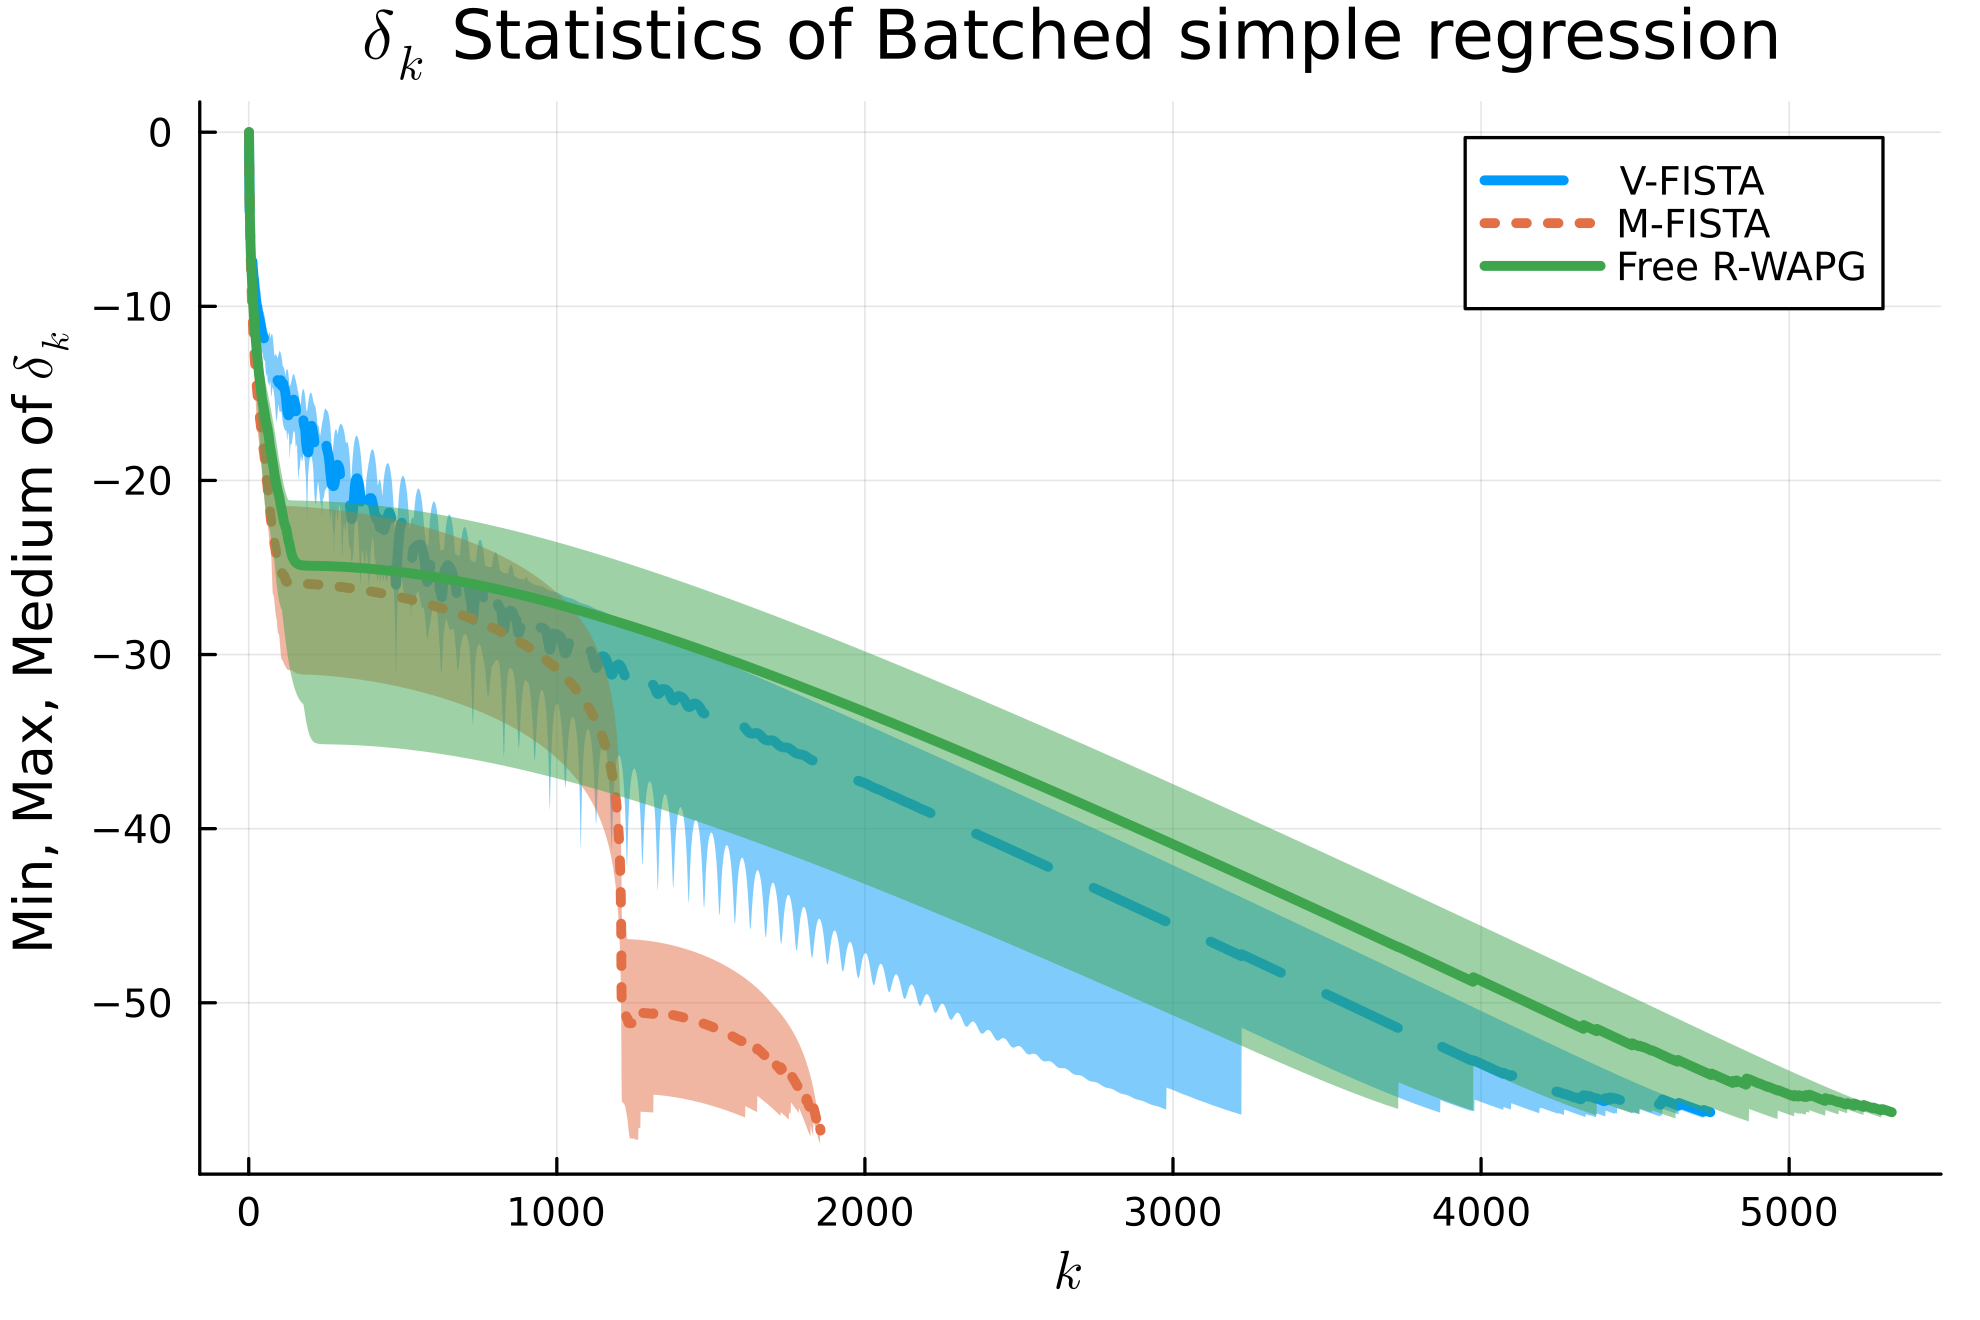
\includegraphics[width=\textwidth]{assets/simple_regression_batched-256.png}
                    \caption{$N = 256$, simple convex quadratic.}
                \end{subfigure}
                \hfill
                \begin{subfigure}[b]{0.47\textwidth}
                    \centering
                    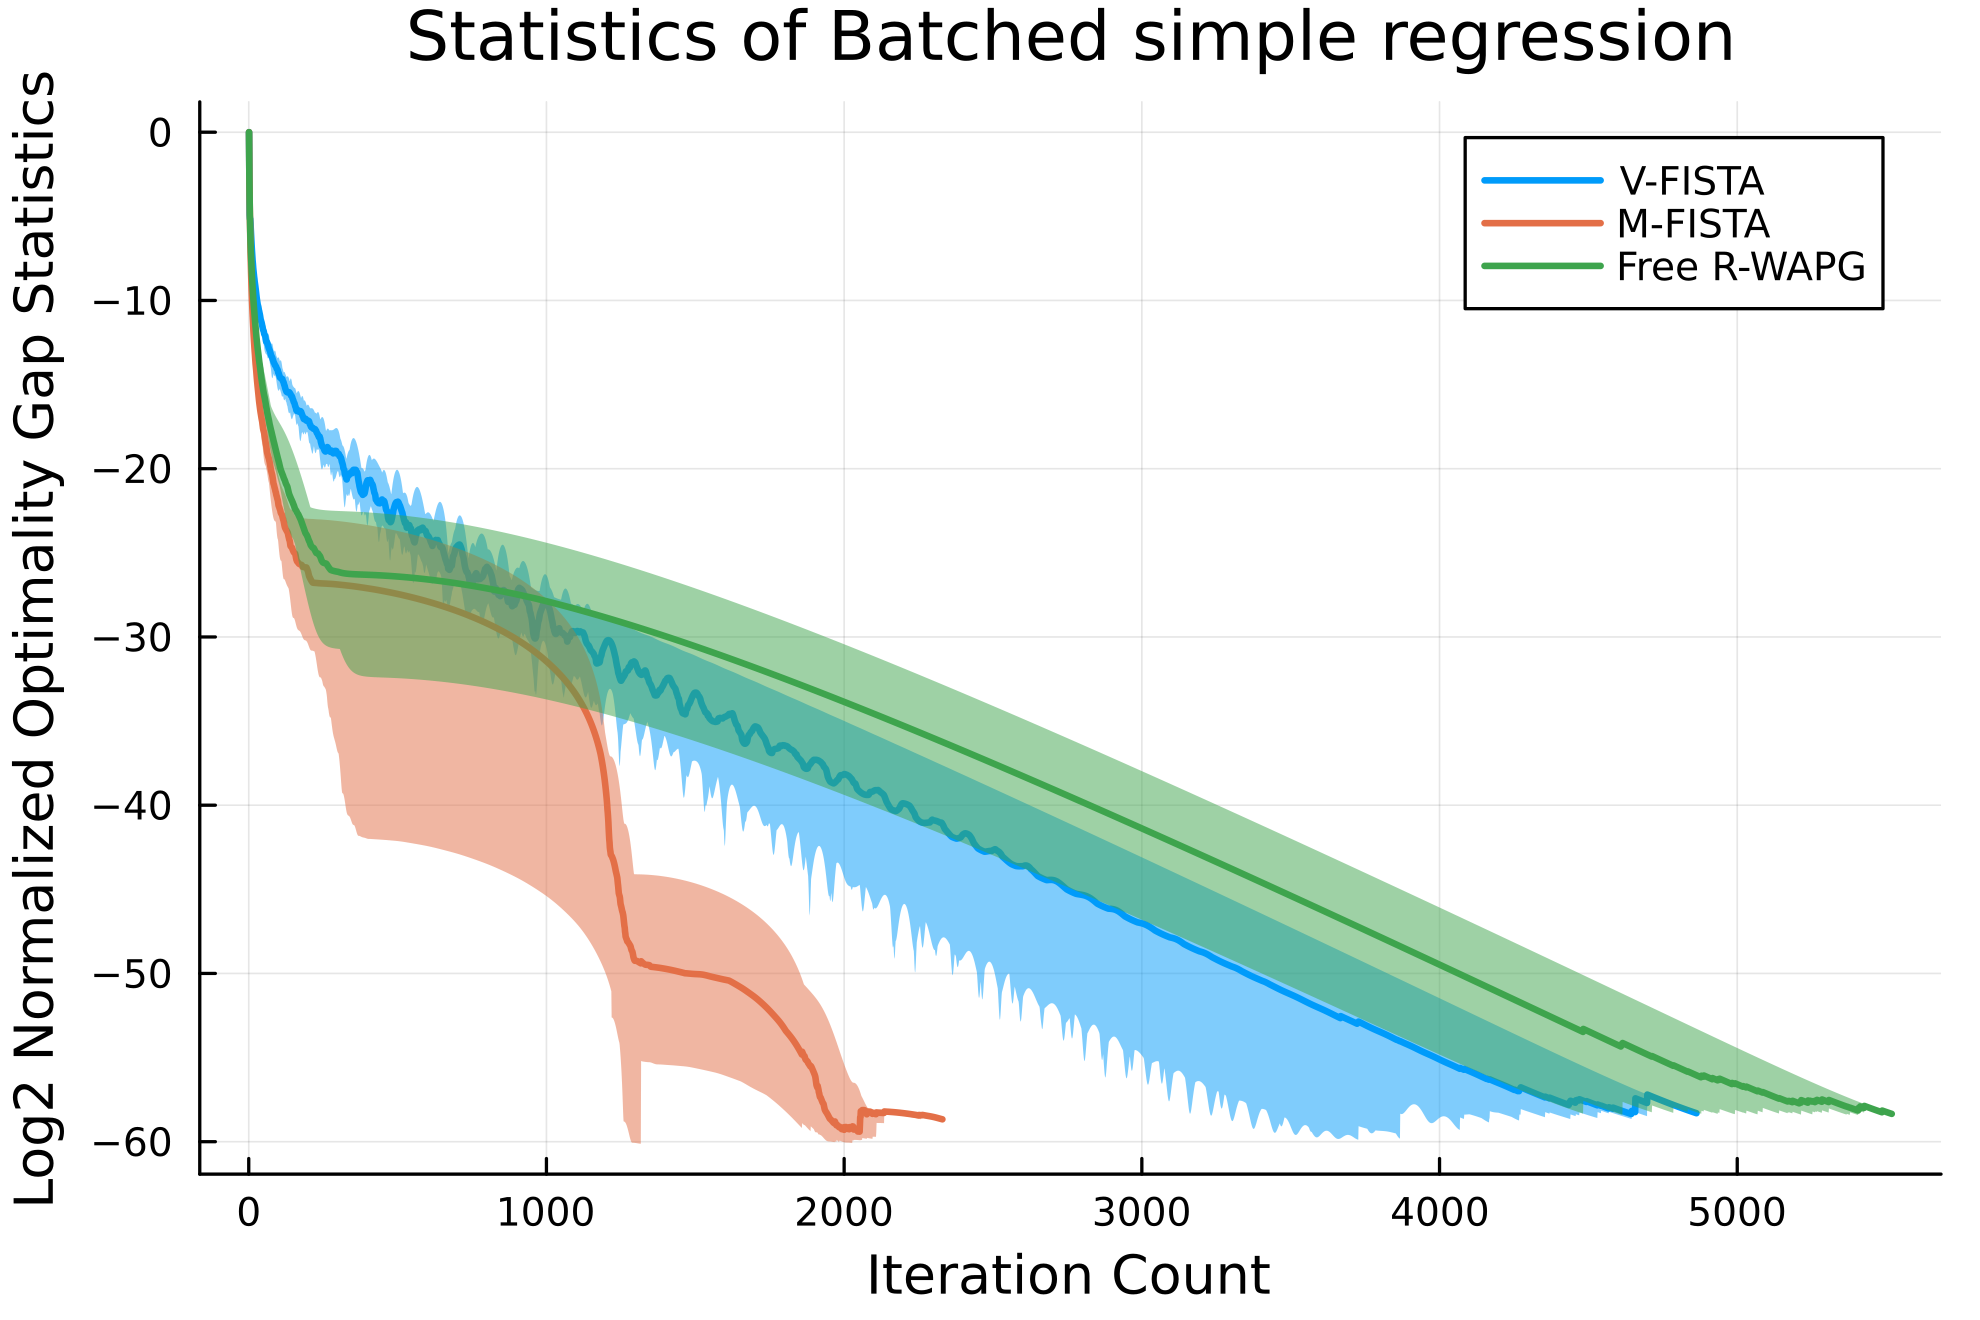
\includegraphics[width=\textwidth]{assets/simple_regression_batched-1024.png}
                    \caption{$N = 1024$, simple convex quadratic. }
                \end{subfigure}
                \caption{Simple convex quadratic experiments results for V-FISTA, M-FISTA, and R-WAPG. }
                \label{fig:simple-quadratic-NOG}
            \end{figure}
        \end{frame}
        \begin{frame}{$\mu$ estimation graph by FR-WAPG}
            FR-WAPG estimates the following for $\mu$ during its execution: 
            \begin{figure}[H]
                \centering
                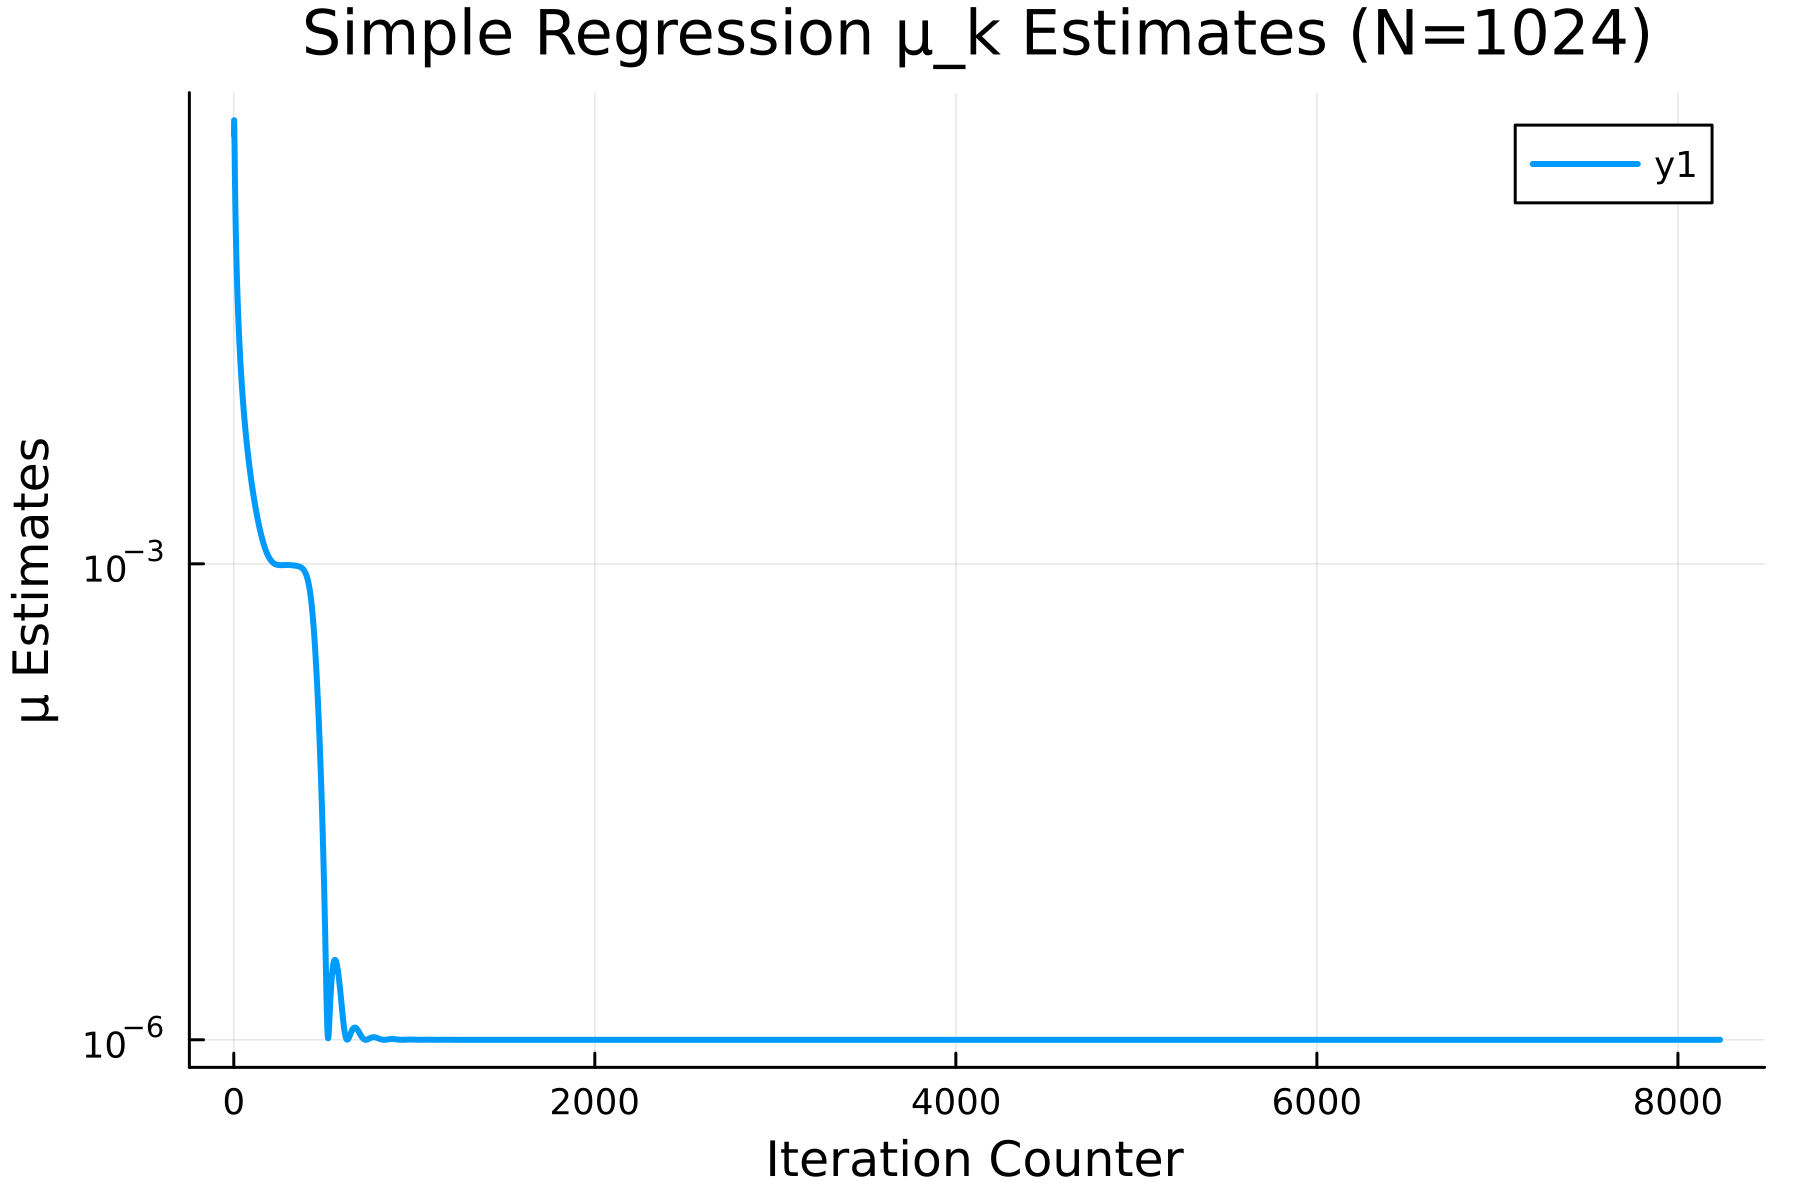
\includegraphics[width=0.64\textwidth]{assets/simple_regression_loss_sc_estimates_1024.png}
                \caption{$N = 1024$, the $\mu$ estimates produced by Algorithm \ref{alg:free-rwapg} (R-WAPG) is recorded. }
                \label{fig:simple-quadratic-r-wapg-mu-estimates}
            \end{figure}
        \end{frame}
        \begin{frame}{LASSO numerical experiment}
            Tibshirani \cite{tibshirani_regression_1996} proposed: 
            \begin{align*}
                \min_x
                \left\lbrace
                    \frac{1}{2}\Vert Ax - b\Vert^2 + \lambda\Vert x\Vert_1
                \right\rbrace. 
            \end{align*}
            Our setup: 
            \begin{enumerate}
                \item $M, N$ are constants. $A \in \RR^{M\times N}$ ahs i.i.d random entries from a standard normal distribution. 
                \item $L, \mu$, are estimated by $A$ by $\mu = 1/\Vert (A^TA)^{-1}\Vert$ and $L = \Vert A^TA\Vert$. 
                \item The synthetic solution is $x^+ = [1\; -1\; 1 \; \cdots ]^T \in \RR^N$ and $b = Ax^+ \in \RR^M$.
                \item $x_0\in \RR^N$ is the initial guess with i.i.d randomed variable from a standard normal distributions. Same initial guess shared by FR-WAPG, V-FISTA, M-FISTA. 
            \end{enumerate}
        \end{frame}
        \begin{frame}{LASSO numerical experiment results}
            Recorded statistics of $\delta_k$ for all algorithms. 
            \begin{figure}[H]
                \begin{subfigure}[b]{0.47\textwidth}
                    \centering
                    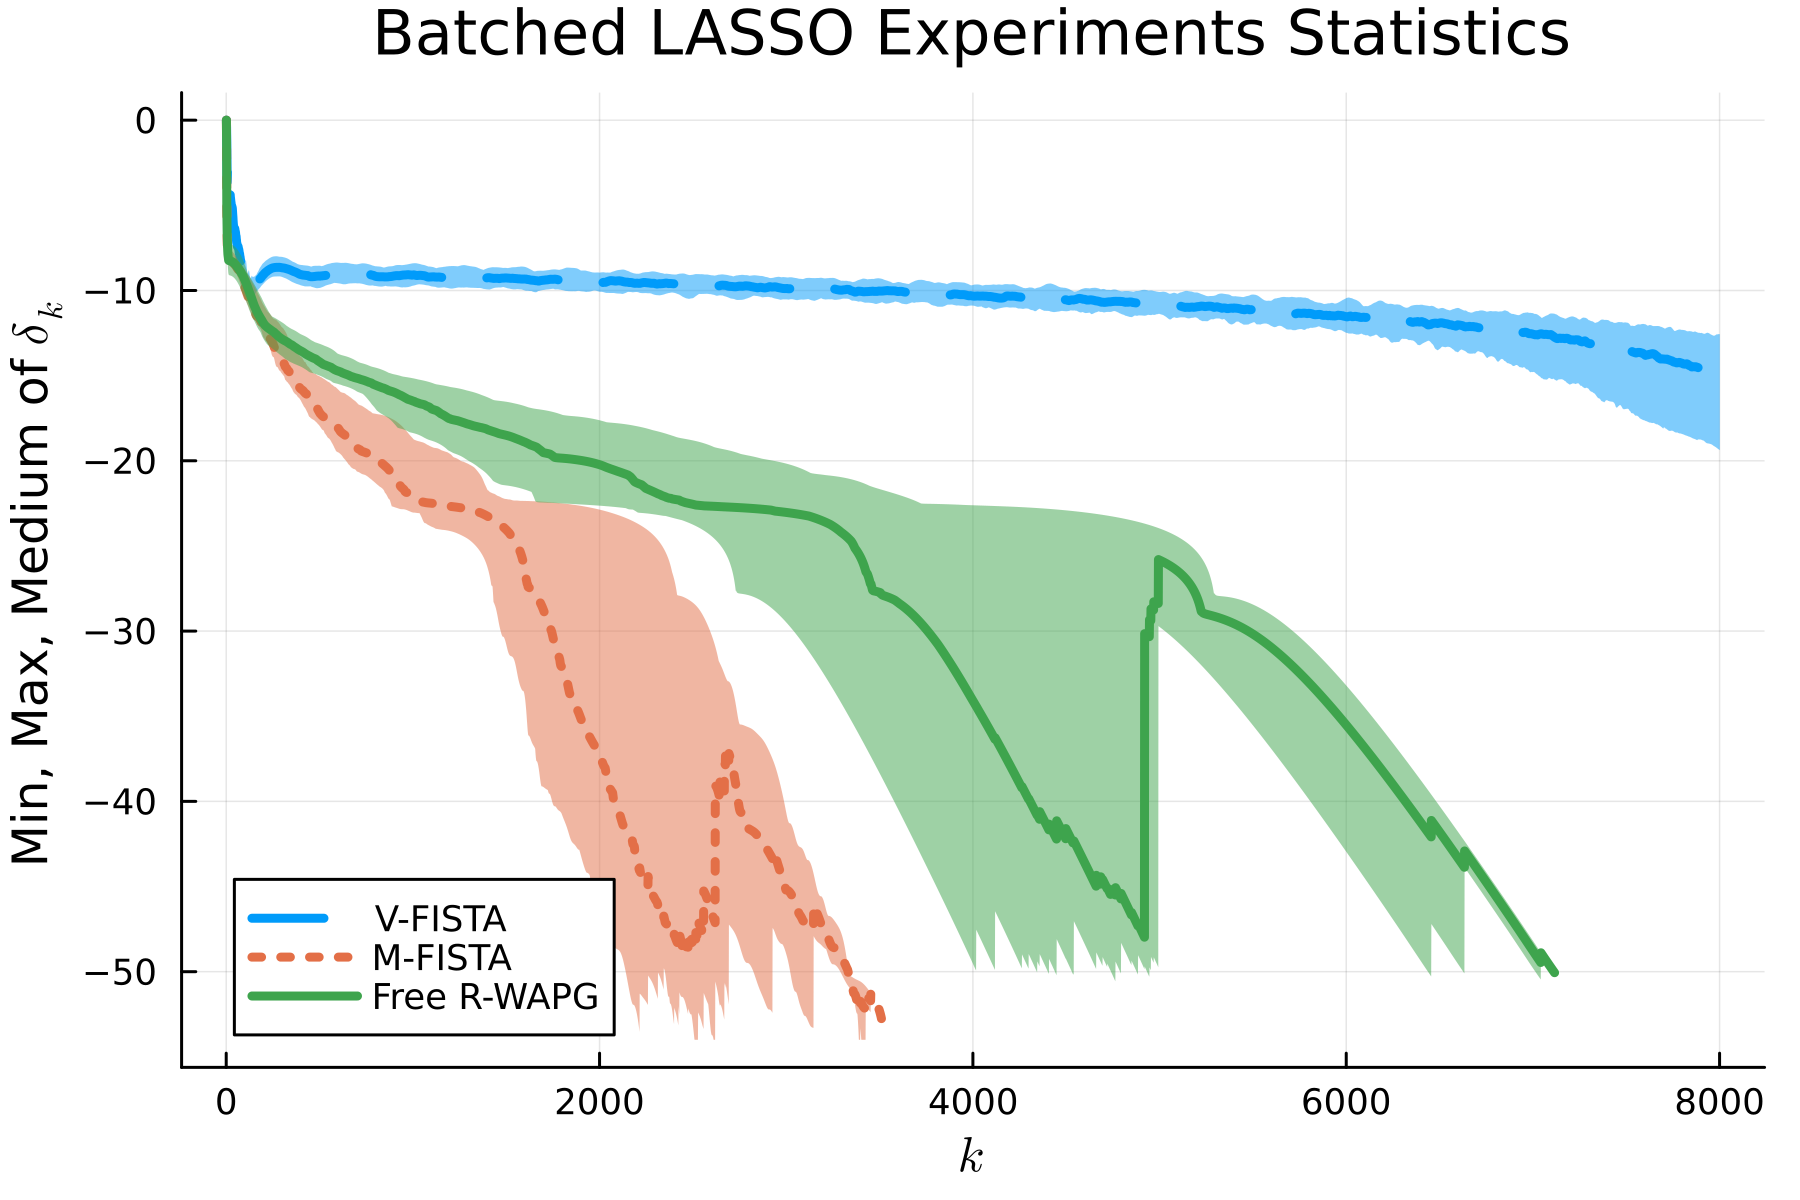
\includegraphics[width=\textwidth]{assets/lasso_batched_statistics_64-256.png}
                    \caption{LASSO experiment with $M = 64, N = 256$. Plots of minimum, maximum, and median $\delta_k$ with estimated $F^*$. }
                \end{subfigure}
                \hfill
                \begin{subfigure}[b]{0.47\textwidth}
                    \centering
                    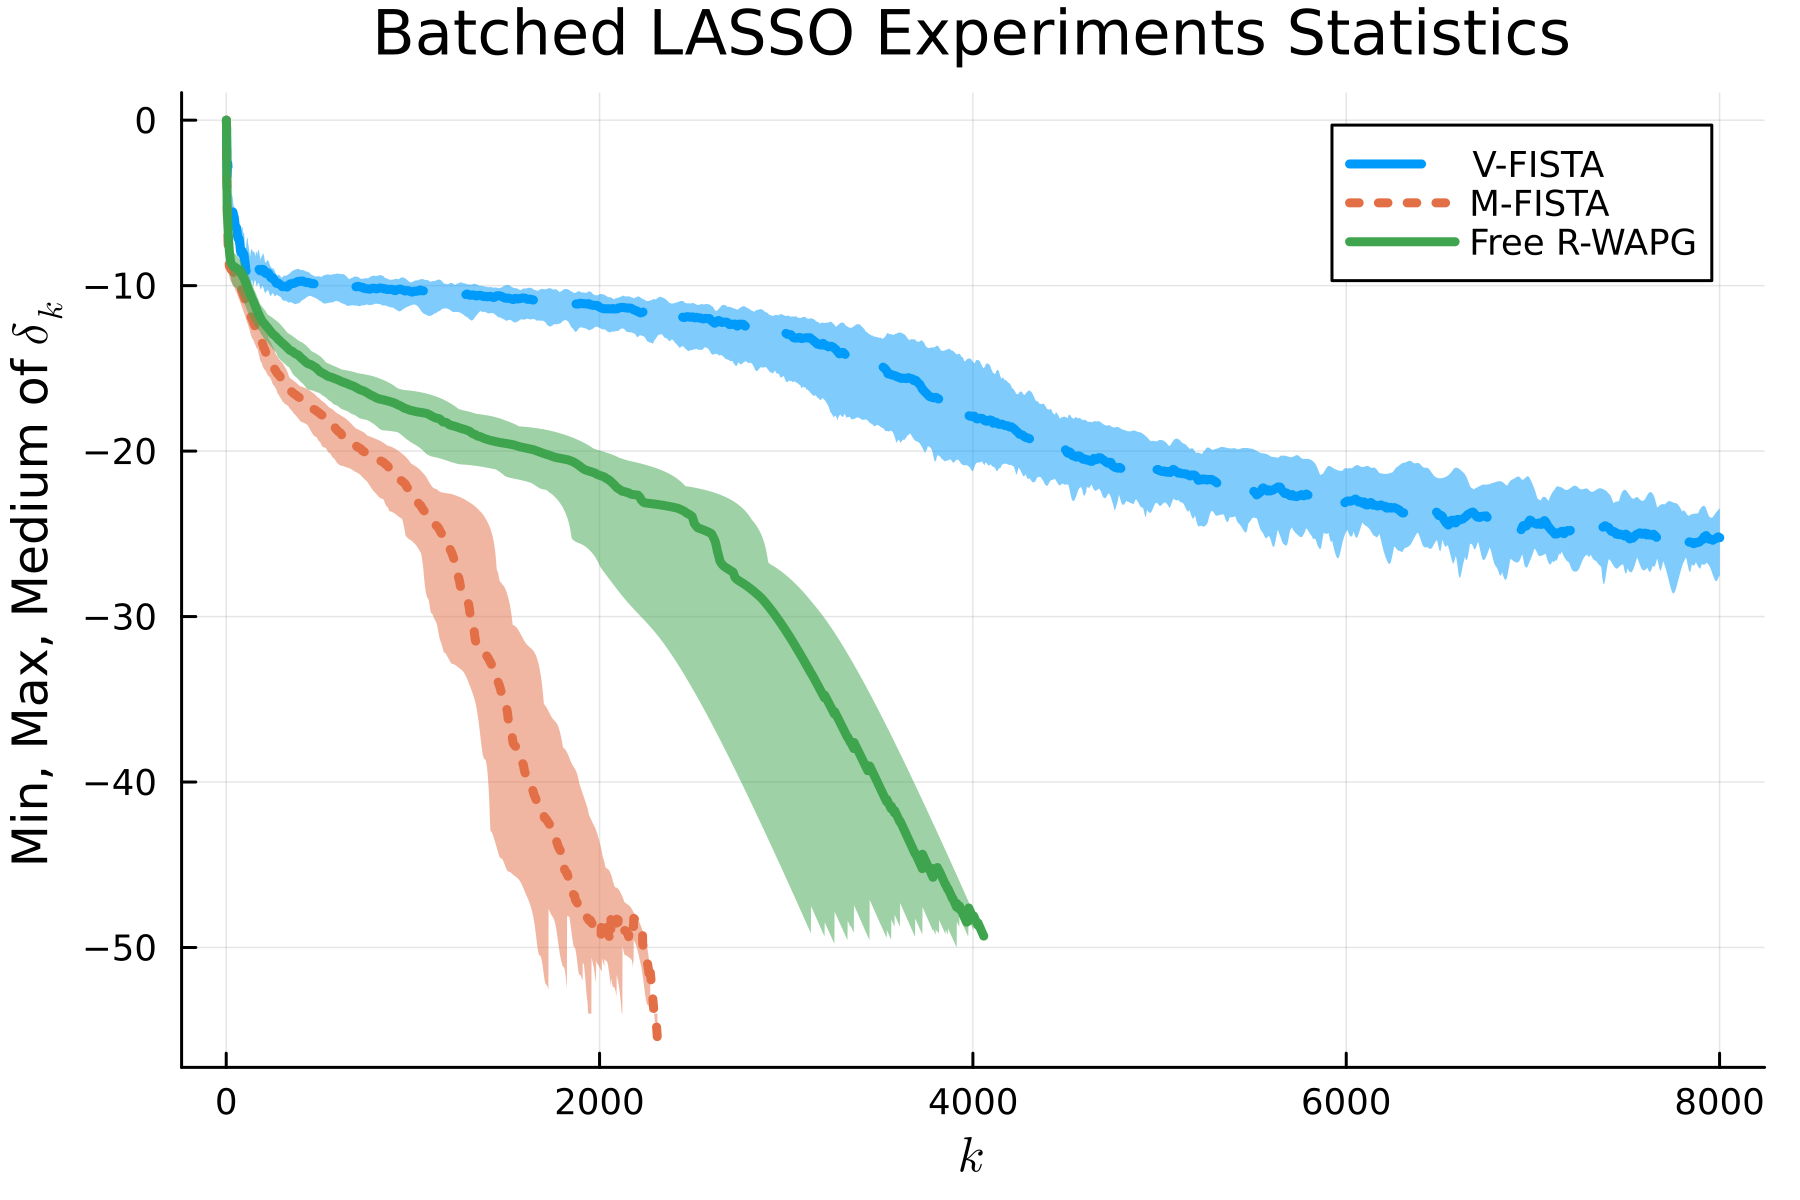
\includegraphics[width=\textwidth]{assets/lasso_batched_statistics_64-128.png}
                    \caption{LASSO experiment with $M = 64, N = 128$. Plots of minimum, maximum, and median $\delta_k$ with estimated $F^*$. }
                \end{subfigure}
                \caption{LASSO experiments. }
                \label{fig:batched-lasso}
            \end{figure}
        \end{frame}
        \begin{frame}{$\mu$ estimates produced from a single LASSO experiment}
            FR-WAPG produces the following estimates for $\mu$ on one of the test instance of LASSO: 
            \begin{figure}[H]
                \begin{subfigure}[b]{0.47\textwidth}
                    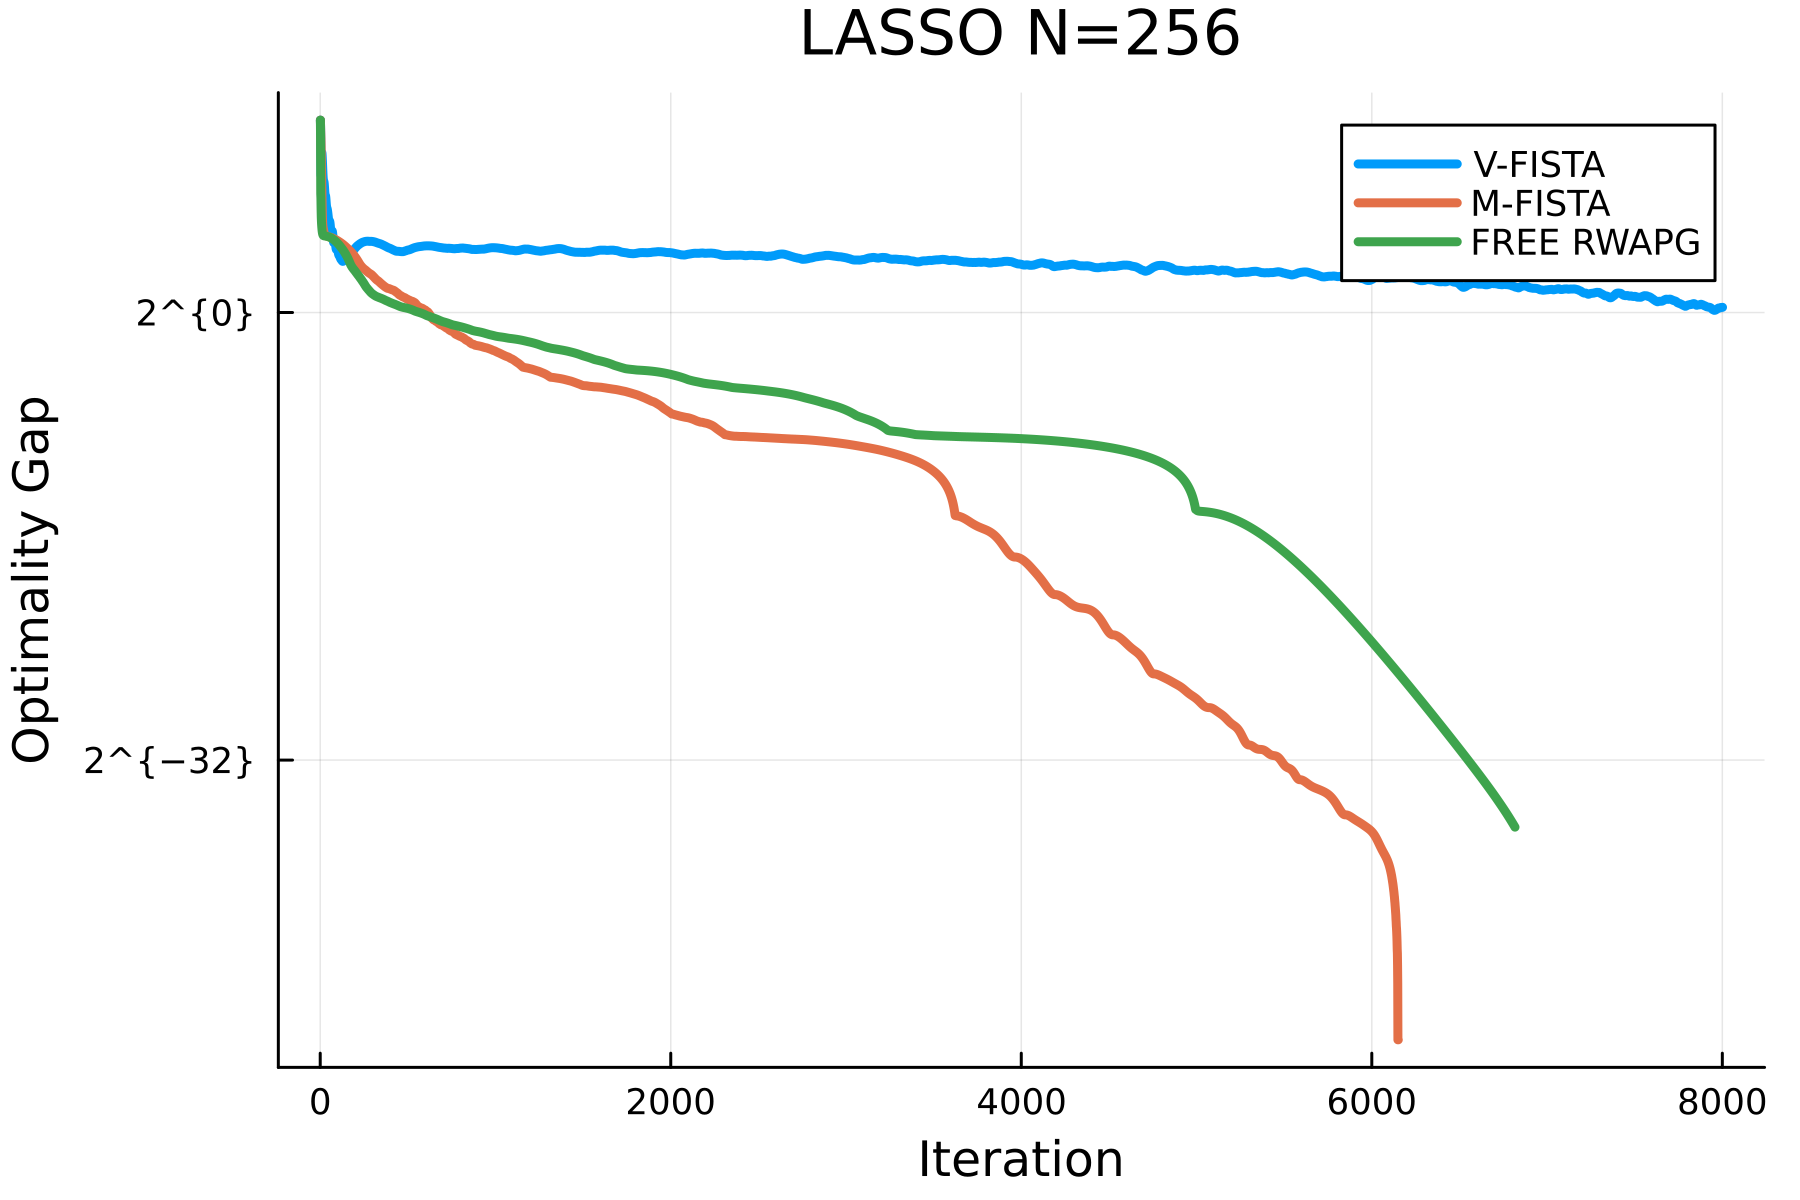
\includegraphics[width=\textwidth]{assets/lasso_loss_256.png}
                    \caption{Single lasso experiment plot of $\delta_k$ with.  }
                \end{subfigure}
                \hfill
                \begin{subfigure}[b]{0.47\textwidth}
                    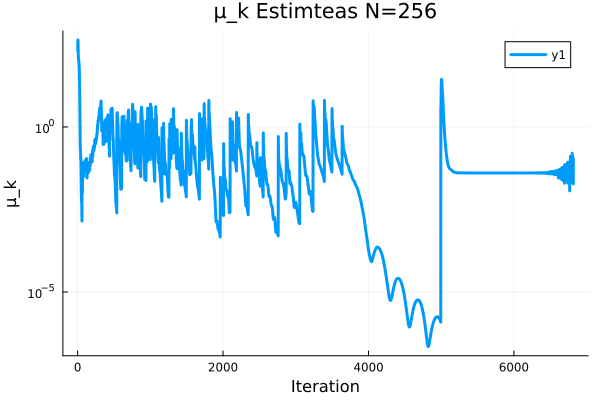
\includegraphics[width=\textwidth]{assets/lasso_sc_estimates_256.png}
                    \caption{The $\mu$ estimated by test algorithms for one LASSO experiment. }
                \end{subfigure}
                \caption{
                    A single LASSO experiment results, with $M = 64, 256$. 
                    We had $\mu = 7.432363627613958\times 10^{-18}$ and $L = 2321.737206983643$.
                }
                \label{fig:single-lass-mu-estimates}
            \end{figure}
        \end{frame}
    \subsection{Direction of future works for R-WAPG}
        \begin{frame}{Nesterov's idea of strong convexity transfer}
            There is one detail that our R-WAPG doesn't incorperate on all Euclidean variants of FISTA. 
            We consider this a minor augmentation for the future. 
            \begin{enumerate}
                \item In Nesterov's 2013 paper \cite{nesterov_gradient_2013}, he considers accelerated  minimization problem $\phi = f + g$ with $f$ $L_f$ smooth and $g$ being $\mu_g \ge 0$ strongly convex. 
                \item Algorithm 5, Chambolle, Pock \cite{chambolle_introduction_2016} captures several variants of FISTA and it assumes that $F = f + g$ where $f, g$ has strong convexity constant $\mu_f \ge 0, \mu_g \ge 0$ respective so $F$ is $\mu := \mu_f + \mu_g \ge 0$ strongly convex. 
            \end{enumerate}
            Fast linear convergence is possible if any one of $f, g$ of the function is strongly convex but this is not yet a prediction of R-WAPG. 
        \end{frame}
        
\section{Selected contents from Catalyst Meta Accelerations}
    \subsection{Introduction to Catalyst}
        \begin{frame}{Assumptions in Catalyst}
            \begin{assumption}\label{ass:catalyst1}
                Given any $\beta > 0$ and $y \in \RR^n$, and $F: \RR^n\rightarrow \overline \RR$ is $\mu \ge 0$ strongly convex and closed. 
                Assume that minimizer exists for $F$ and the minimum is $F^*$. 
                For all $x,y\in \RR^n, \beta > 0$ define the model function: 
                \begin{align*}
                    \mathcal M^{\beta^{-1}}_F(x; y) &:= 
                    F(x) + \frac{\beta}{2}\Vert x - y\Vert^2.
                \end{align*}
                We define the Moreau Envelope at $y \in \RR^n$ to be $\mathcal M^*_{F,\beta^{-1}}(y) := \min_{x\in \RR^n} \mathcal M_F^{\beta^{-1}}(x; y)$. 
                We denote $\mathcal J_{\beta^{-1}F}$ to be the resolvent operator for subgradient of $F$, which is also called the proximal operator. 
            \end{assumption}
        \end{frame}
        \begin{frame}{Absolute termination criterion}
            \begin{definition}[Absolute termination criterion C1]\label{def:catalyst-termination-c1}
                Take $F$ as given by Assumption \ref{ass:catalyst1}.
                For $\epsilon > 0, \kappa > 0$ and $x \in \RR^n$, the absolute criterion C1 characterizes the set of inexact proximal iterates by: 
                \begin{align*}
                    \mathcal J_{\kappa^{-1} F}^\epsilon (x) := 
                    \left\lbrace
                        y \in \RR^n \left | \; 
                                \mathcal M^{1/\kappa}_F (y; x) - 
                                \mathcal M^*_{F, 1/\kappa}(x) \le \epsilon
                        \right.
                    \right\rbrace. 
                \end{align*}
            \end{definition}
            \begin{definition}[Relative termination criterion C2]\label{def:catalyst-termination-c2}
                Take $F$ as given by Assumption \ref{ass:catalyst1}. 
                Given any $\delta \in (0, 1]$, $\kappa > 0$ and $x \in \RR^n$, the relative criterion C2 of the inexact resolvent is defined by: 
                {\small
                \begin{align*}
                    \widetilde{\mathcal J}_{\kappa^{-1}F}^\delta (x)
                    := 
                    \left\lbrace
                        z \in \RR^n \left| \;
                            \mathcal M_F^{\kappa^{-1}}(z; x) - 
                            \mathcal M^*_{F, \kappa^{-1}}(z; x)
                            \le \frac{\kappa\delta}{2}\Vert x - z\Vert^2
                        \right.
                    \right\rbrace. 
                \end{align*}
                }
            \end{definition}
        \end{frame}
        \begin{frame}{Catalyst meta acceleration}
            \begin{definition}[Lin's Universal Catalyst Acceleration]\label{def:lin-catalyst-original}
                Let $F:\RR \rightarrow \overline \RR$ be $\mu \ge 0$ strongly convex and closed. 
                Let the initial estimate be $x_0 \in \RR^n$, fix parameters $\kappa > 0$ and $\alpha_0 \in (0, 1]$. 
                Let $(\epsilon_k)_{k \ge 0}$ be an absolute error sequence chosen for the evaluation for inexact proximal point method. 
                {\small
                \begin{tcolorbox}
                    Initialize $x_0 = y_0$. Then the algorithm generates $(x_k, y_k)_{k\ge 0}$ for all $k \ge 1$ such that: 
                    \begin{align*}
                        & \text{find } x_k \in \mathcal J_{\kappa^{-1}F}^{\epsilon_k} y_{k - 1}, 
                        \\
                        & \text{find } \alpha_k \in (0, 1) \text{ such that } \alpha_k^2 = (1 - \alpha_k)\alpha_{k - 1}^2 + (\mu/(\mu + \kappa))\alpha_k,
                        \\
                        & 
                        y_{k} = x_k + \frac{\alpha_{k - 1}(1 - \alpha_{k - 1})}{\alpha_{k - 1}^2 + \alpha_k}(x_k - x_{k - 1}). 
                    \end{align*}
                \end{tcolorbox}
                }
            \end{definition}
            Denotes the outerloop algorithm, i.e: Definition \ref{def:lin-catalyst-original} by $\mathbb A$, denote the inner loop algorithm by $\mathbb M$. 
        \end{frame}
    \subsection{Complexity theoreis with absolute errors}
        \begin{frame}{Inner loop complexity assumption}
            The following assumption is crucial and we will return to it. 
            \begin{assumption}[Linear convergence of inner loop]\label{ass:linear-convergence-inner-loop}
                For any $k \in \N$, $y \in \RR^n$. 
                Suppose $\mathbb M$ generates iterates $(z_{k, t})_{t \ge 0}$ for the inner loop iteration such that there exists $A > 0$, and it has: 
                {\small
                \begin{align*}
                    \mathcal M_F^{\kappa^{-1}}(z_{k, t}, y) - \mathcal M^*_{F, \kappa^{-1}}(y) 
                    &\le 
                    A(1 - \tau_{\mathbb M})^t
                    \left(
                        \mathcal M_{F}^{\kappa^{-1}}(z_{k,0})
                        -
                        \mathcal M^*_{F, \kappa^{-1}}(y)
                    \right). 
                \end{align*}
                }
            \end{assumption}
        \end{frame}
        \begin{frame}{Outer loop complexity, strong convex case}
            \begin{theorem}[]\label{thm:err-seq-outer-s-cnvx}
            {\small
                For $\mathbb A$ with regularization parameter $\kappa > 0$. 
                Assume that $F$ is $\mu > 0$ strongly convex. 
                Choose $\alpha_0 = \sqrt{q}$ with $q = \mu/(\kappa + \mu)$ and the absolute error sequence 
                $$
                \begin{aligned}
                    \epsilon_k = \frac{2}{9}(F(x_0) - F^*)(1 - \rho)^k \quad \text{with }\quad 
                    \rho < \sqrt{q}. 
                \end{aligned}
                $$
                Then the $\mathbb A$ generates $(x_{k})_{k \ge 0}$ such that 
                $$
                \begin{aligned}
                    F(x_k) - F^* &\le 
                    C(1 - \rho)^{k + 1} (F(x_0) - F^*) \quad \text{ with }\quad 
                    C = \frac{8}{(\sqrt{q} - \rho)^2}. 
                \end{aligned}
                $$
            }
            \end{theorem}
        \end{frame}
        \begin{frame}{Outer loop complexity, convex but not strongly convex case}
            \begin{theorem}[]\label{thm:erro-seq-outer-cnvx}
            {\small
                For $\mathbb A$ with regularization parameter $\kappa > 0$. 
                Assume that $F$ is convex but with strong convexity constant $\mu = 0$. 
                Choose $\alpha_0 = (\sqrt{5} - 1)/2$ and the absolute error sequence 
                \begin{align*}
                    \epsilon_k &= \frac{2(F(x_0) - F^*)}{9(k + 2)^{4 + \eta}} \quad 
                    \text{with}\quad \eta > 0. 
                \end{align*}
                Take $x^*$ to be a minimizer of $F$. 
                Then algorithm $\mathbb A$ generates $(x_k)_{k \ge0}$ such that it has a convergence rate of 
                \begin{align*}
                    F(x_k) - F^* &\le 
                    \frac{8}{(k + 2)^2}\left(
                        \left(1 + \frac{2}{\eta}\right)^2(F(x_k) - F^*)
                        + \frac{\kappa}{2}\Vert x_0 - x^*\Vert^2
                    \right).
                \end{align*}
            }
            \end{theorem}
        \end{frame}
        \begin{frame}{Inner loop complexity, absolute errors}
            \begin{proposition}[Inner loop complexity strongly convex]\label{prop:inner-loop-complexity-s-cnvx}
            {\footnotesize
                Under the same settings of Theorem \ref{thm:err-seq-outer-s-cnvx}, suppose that 
                \begin{enumerate}
                    \item $\mathbb M$ has linear convergence rate as specified in Assumption \ref{ass:linear-convergence-inner-loop}, 
                    \item $\mathbb M$ is initialized with  $z_{k, 0} = x_{k - 1}$ for all $k \ge 2$. 
                \end{enumerate}
                Then, the precision $\epsilon_k$ is achieved within at most a number of iteration $T_{\mathbb M} \le \widetilde {\mathcal O}(1/ \tau_{\mathbb M})$. 
                Here $\widetilde{\mathcal O}$ hides logarithmic complexity in $\mu, \kappa$ and other constants. 
            }
            \end{proposition}
            \begin{proposition}[Inner loop, context but not strongly convex]\label{prop:inner-loop-complexity-cnvx}
            {\footnotesize
                Under the settings of Theorem \ref{thm:erro-seq-outer-cnvx}, suppose that:
                \begin{enumerate}
                    \item $\mathbb M$ has linear convergence rate as specified in Assumption \ref{ass:linear-convergence-inner-loop}, 
                    \item the initial guess for $\mathbb M$ is $z_{0, k} = x_{k - 1}$, 
                    \item $F$ has bounded level set.
                \end{enumerate}
                Then there exists $T_{\mathbb M} \le \widetilde{\mathcal O}(1 / \tau_{\mathbb M})$ such that for any $k \ge 1$, it requires at most\\ $T_{\mathbb M}\log(k + 2)$ iterations for $\mathbb M$ to achieve accuracy $\epsilon_k$.
            }
            \end{proposition}
        \end{frame}

        \begin{frame}{Aggregated complexity}
            We count $m$, the number of iteration experienced by $\mathbb M$ for the $k$ th iteration of $\mathbb A$. 
            \begin{enumerate}
                \item If $\mu > 0$, \ref{prop:inner-loop-complexity-s-cnvx} gives $m \le T_{\mathbb M}k$. 
                Substituting $k \ge m/T_{\mathbb M}$ into Theorem \ref{thm:err-seq-outer-s-cnvx}: 
                {\footnotesize
                \begin{align*}
                    F(x_k) - F^* &\le \mathcal O \left(
                        (1 - \rho)^k 
                    \right) \le 
                    \mathcal O \left(
                        (1 - \rho)^{m/ T_{\mathbb M}}
                    \right) \le 
                    \mathcal O\left(
                        \left(1 - \rho/T_{\mathbb M}\right)^{m}
                    \right)
                    \\
                    &\le \widetilde{\mathcal O}\left(
                        \tau_{\mathbb M}\sqrt{\mu}/(\mu + \kappa)
                    \right). 
                \end{align*}
                }
                \item If $\mu = 0$, using Proposition \ref{prop:inner-loop-complexity-cnvx}, Theorem \ref{thm:erro-seq-outer-cnvx} it has 
                {\footnotesize
                \begin{align*}
                    m &\le \sum_{i - 1}^{k} k T_{\mathbb M} \log(i + 2) \le k T_{\mathbb M} \log(k + 2) 
                    \le T_{\mathbb M}k(k + 2) 
                    \le 
                    \mathcal O(T_{\mathbb M} k^2). 
                \end{align*}
                So: 
                \begin{align*}
                    F(x_k)- F^* &\le 
                    \mathcal O(k^{-2})\le 
                    \mathcal O
                        \left(
                            m^{-2}T_{\mathbb M}
                        \right) 
                        \le \widetilde{\mathcal O}
                            \left(m^{-2}\tau_{\mathbb M}^{-1}\right). 
                \end{align*}
                }
            \end{enumerate}
        \end{frame}
    \subsection{Complexity theories with relative errors}
        \begin{frame}{Catalyst acceleration with relative errors}
            \begin{definition}[Catalyst Acceleration with relative error]\label{def:catalyst-relative}
            {\small
                Let $F:\RR \rightarrow \overline \RR$ be $\mu \ge 0$ strongly convex and closed. 
                Let the initial estimate be $x_0 \in \RR^n$, fix parameters $\kappa > 0$ and $\alpha_0 \in (0, 1]$. 
                Let $(\delta_k)_{k \ge 0}$ be an absolute error sequence chosen for the evaluation for inexact proximal point method. 
                \begin{tcolorbox}
                    Initialize $x_0 = y_0$. Then the algorithm generates $(x_k, y_k)_{k\ge 0}$ for all $k \ge 1$ such that: 
                    \begin{align*}
                        & \text{find } x_k \in \widetilde{\mathcal J}_{\kappa^{-1}F}^{\delta_k} y_{k - 1}, 
                        \\
                        & \text{find } \alpha_k \in (0, 1) \text{ such that } \alpha_k^2 = (1 - \alpha_k)\alpha_{k - 1}^2 + (\mu/(\mu + \kappa))\alpha_k,
                        \\
                        & 
                        y_{k} = x_k + \frac{\alpha_{k - 1}(1 - \alpha_{k - 1})}{\alpha_{k - 1}^2 + \alpha_k}(x_k - x_{k - 1}). 
                    \end{align*}
                \end{tcolorbox}
            }
            \end{definition}
        \end{frame}
        \begin{frame}{Outerloop complexity under relative errors}
            \begin{theorem}[Outer loop complexity under criterion C2]\label{theorem:catalyst2-outer-loop}
                For the iterates $(x_k)_{k \ge 0}$ generated by algorithm in Definition \ref{def:catalyst-relative}, we have 
                \begin{enumerate}
                    \item If $\mu > 0$, choose $\alpha_0 = \sqrt{q}$, $\delta_k = \sqrt{q}/(2 - \sqrt{q})$. 
                    Then the iterates $(x_k)_{k \ge 0}$ satisfies $F(x_k) - F^* \le \mathcal O\left(1 - \sqrt{q}/2\right)^k$. 
                    \item If $\mu = 0$, choose $\alpha_0 = 1$, $\delta_k = 1/(k + 1)^2$ satisfies $F(x_k) - F^* \le \mathcal O(k^{-2})$. 
                \end{enumerate}
            \end{theorem}
            \begin{remark}
                This is Proposition 8, 9 in Lin et al.'s second Catalyst paper \cite{lin_catalyst_2018}.
                For a precise description of the upper bound, see Theorem 8. 
            \end{remark}
            Observe that it does't require knowledge about $F^*$. 
        \end{frame}


    \subsection{Direction of future works}


\section{References}
    \begin{frame}{Citation examples}
        Citation examples \cite{chambolle_convergence_2015}
    \end{frame}

    \begin{frame}[allowframebreaks]{References}
        % \bibliographystyle{apalike}
        \bibliography{references/proposal.bib}
    \end{frame}

\end{document}